\documentclass{article}
\usepackage{graphicx}
\usepackage{amsmath}
\usepackage[margin=1in]{geometry}
\usepackage{bm}

\renewcommand{\vec}[1]{\bm{#1}}
\newcommand{\del}{\partial}

\author{Michael Bentley}
\title{Project 4: CasADi playing}
\date{05 Feb 2019}

\begin{document}
\maketitle

CasADi is a symbolic framework for nonlinear optimization and algorithmic
differentiation.
%
Here we use CasADi not as intended.
%
We are using it as a gateway to utilizing the nonlinear optimization solvers it
employs.
%
However, CasADi is targeted to solving optimal control problems.


\section{Reaching Desired Task Space Positions}

This is all about reaching the goal.

\subsection{}

\begin{figure}
  \centering
  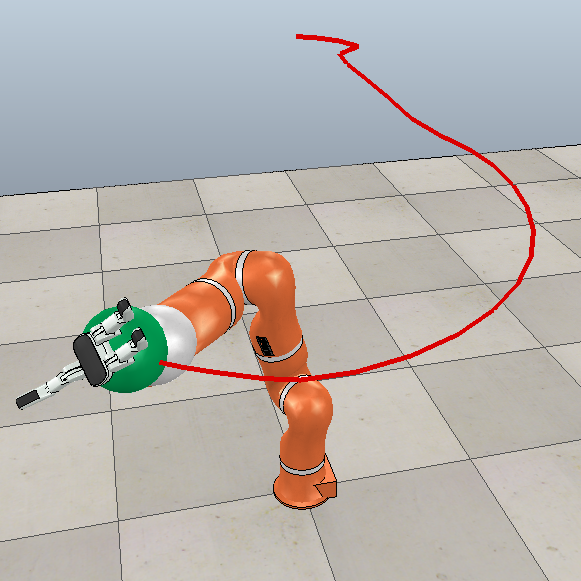
\includegraphics[width=.3\textwidth]{images/p1-1-1.png} \hspace{1em}
  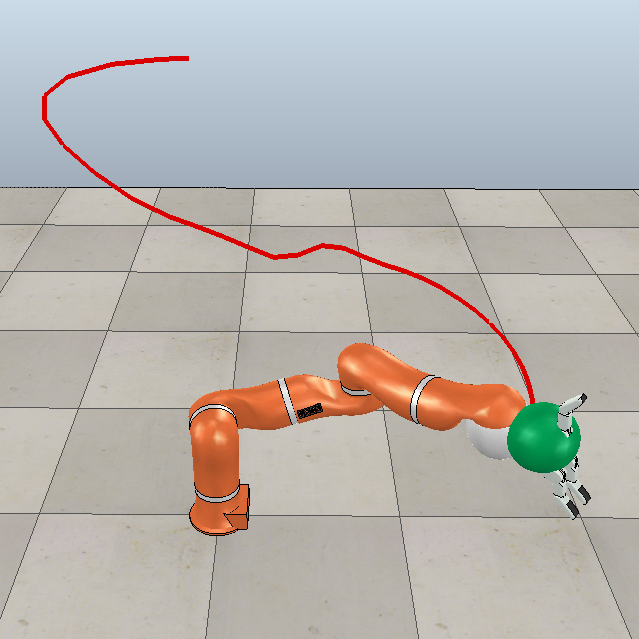
\includegraphics[width=.3\textwidth]{images/p1-1-2.png} \hspace{1em}
  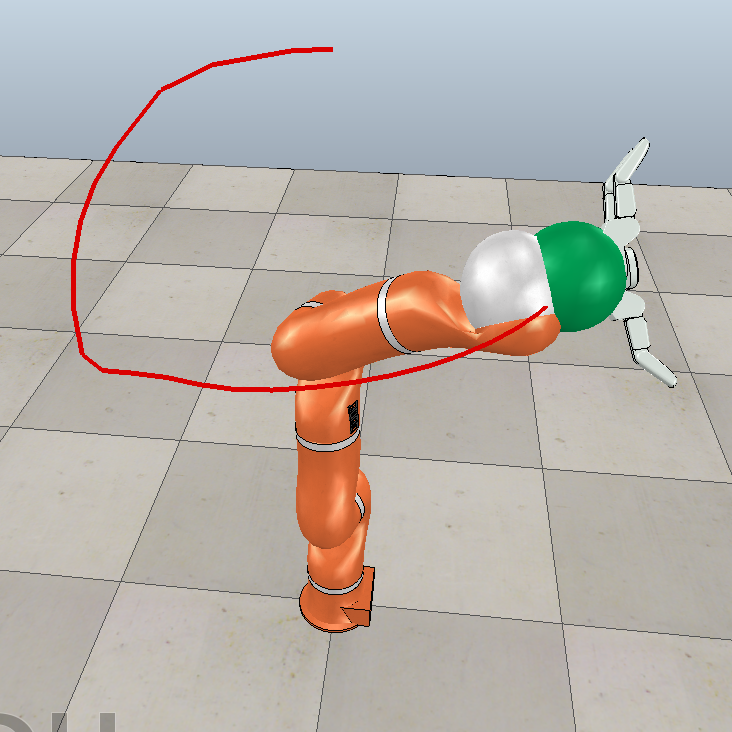
\includegraphics[width=.3\textwidth]{images/p1-1-3.png}
  \caption{
    Screenshots of three executions of problem 1.1 using randomly generated
    goal locations.
    }
  \label{fig:p1.1-screenshots}
\end{figure}

We are to implement the following optimization problem:

\begin{align*}
  \min_{\vec{\theta}}
    & \quad
      \sum_{t = 1}^T
      ||
      FK(\vec{\theta}_t) - \vec{x}_g
      ||^2_2
  \\
  \text{s.t.}
    & \quad
      \vec{\theta}_{lower}
        \leq
      \vec{\theta}_t
        \leq
      \vec{\theta}_{upper}
  \\
    & \quad
      t = 1, \ldots, T.
\end{align*}

This was implemented and run three times.
%
In Figure~\ref{fig:p1.1-screenshots}, we see the screenshots after the three
executions with randomly generated goal locations.
%
Sometimes the robot has a very direct trajectory, which makes sense, as that
would reduce the cost function.
%
However, other times, it takes a seemingly indirect approach.
%
I believe this has to do with the joint limits and having to go around the long
way based on some goal locations.
%
Also, I observe that the trajectories are pretty fast, which is nice.


\subsection{}

Here we add an inequality constraint to the optimization problem of 1.1 to
limit joint velocity.
%
The following constraints are added to 1.1:
%
\begin{align*}
  -\gamma \leq \theta_{i,t} - \theta_{i,t - 1} \leq \gamma,
    ~
    \forall \theta_i
  \\
  FK(\vec{\theta}_T) = \vec{x}_g
  \\
  \dot{\vec{\theta}}_T = 0
\end{align*}
%
With these added constraints, the optimization took many more iterations before
converging.
%
This made the optimization much less tractable for real-time applications.
%
Each execution tool about a full minute to complete for a single trajectory
without obstacle avoidance.


As for the difference between the trajectories generated in 1.1 and 1.2, I
observe that the trajectory is much smoother and slower.
%
It seems like a trajectory that I would trust to be able to control on a real
robot.



\subsection{}

We add a smoothness term to the objective function and see how that effects
things:
%
\begin{equation*}
  f(\vec{\theta}_t, \vec{\theta}_{t-1}, \vec{x}_g)
    =
      ||
        FK(\vec{\theta}_t)
        -
        \vec{x}_g
      ||_2^2
      +
      \alpha
      ||
        \vec{\theta}_t
        -
        \vec{\theta}_{t-1}
      ||_2^2
\end{equation*}

I did this, but I don't feel like finishing the report here.
%
I just played with it some more.


What was curious here is that when the end effector was far away from the goal,
the arm moved very quickly, but as it got closer, the arm moved slower and
slower.
%
I tried raising the alpha value, but that just makes it go even slower the
closer it gets to the goal position.
%
I'm not sure this is the best approach for this.
%
Perhaps it would be better to, instead of penalizing velocity, only penalizing
velocity above a certain threshold.
%
Although, an approach that has a threshold for velocity is more similar to the
second approach where the hard constraints are turned into soft constraints
(which is how many optimization frameworks work anyway).


\section{Obstacle Avoidance}

\subsection{}

The objective function I would like to use that also avoids the obstacle
located at $\vec{x}_{obst}$ is
%
\begin{equation*}
  f(\vec{\theta}_t, \vec{x}_g, \vec{x}_{obst})
    =
      ||FK(\vec{\theta}_t) - \vec{x}_g||_2^2
      +
      \frac{
        \beta
      }{
        ||FK(\vec{\theta}_t) - \vec{x}_{obst}||_2^2
      }
\end{equation*}

\subsection{}

\begin{figure}
  \centering
  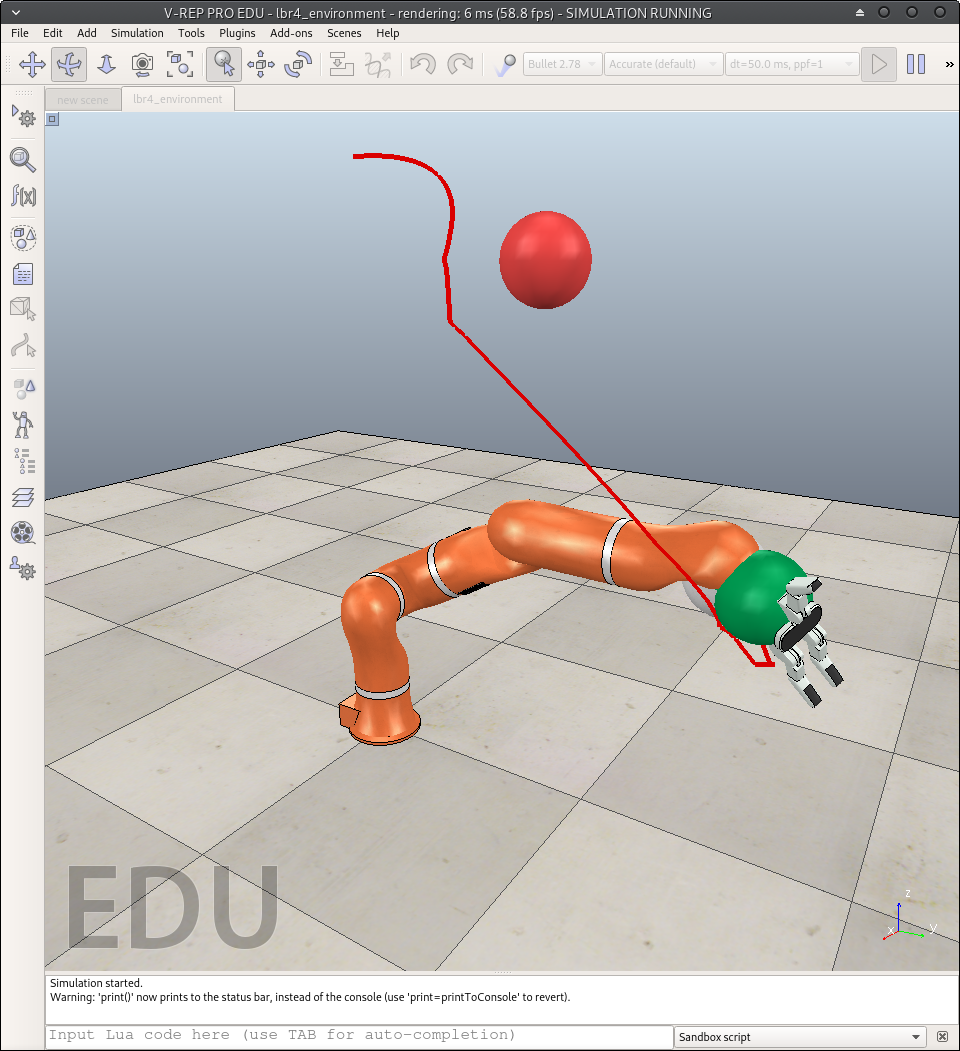
\includegraphics[width=0.3\textwidth]{images/p2-2-1.png} \hspace{1em}
  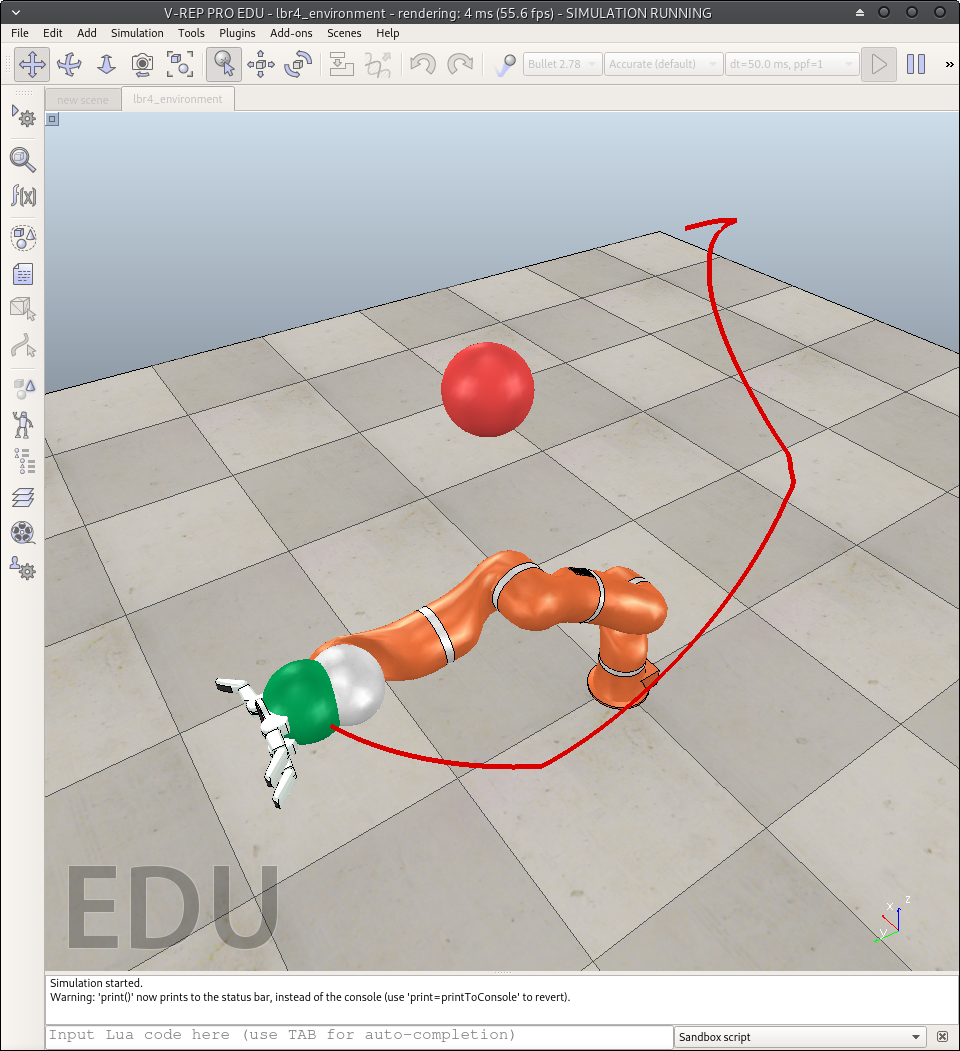
\includegraphics[width=0.3\textwidth]{images/p2-2-2.png} \hspace{1em}
  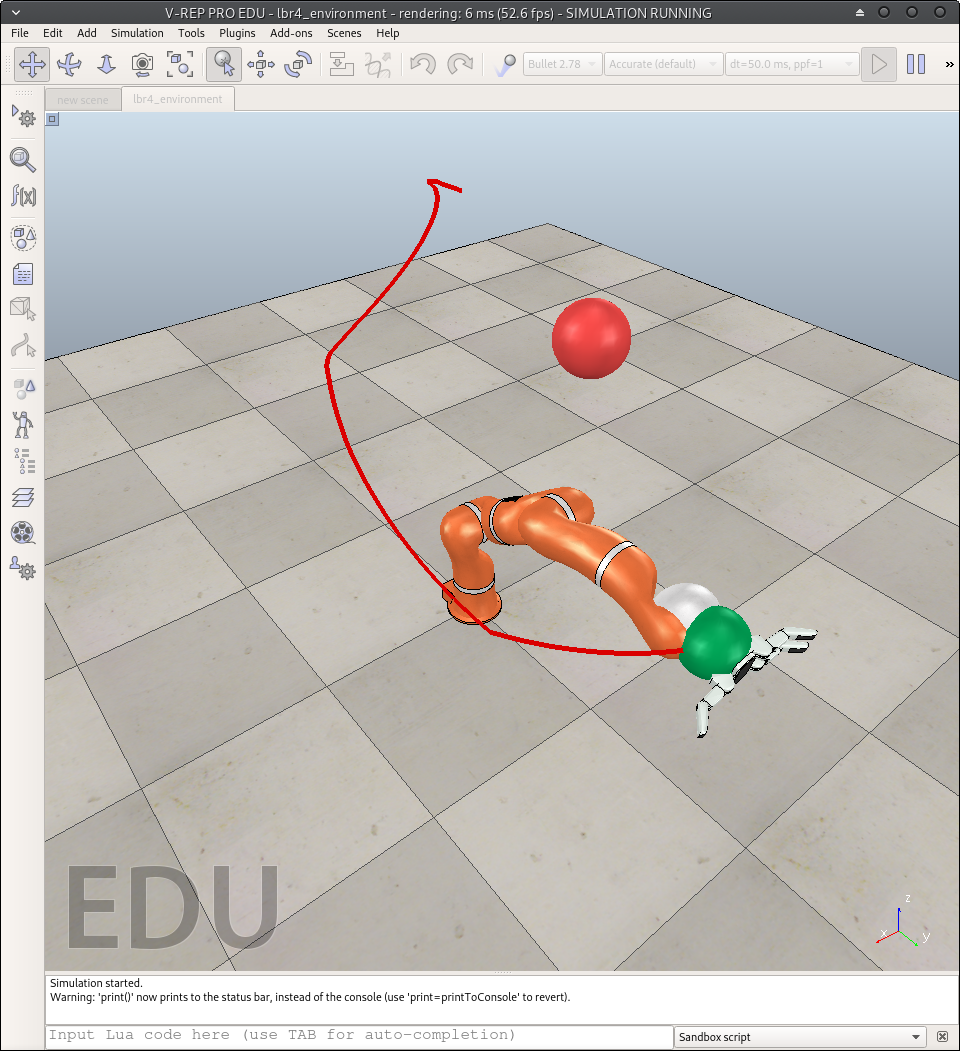
\includegraphics[width=0.3\textwidth]{images/p2-2-3.png}
  \caption{Left: $\beta = 0.05$, Middle: $\beta = 1$, Right: $\beta = 10$}
  \label{fig:p2-2}
\end{figure}

\subsection{}


\end{document}
